\documentclass[10pt,a4paper,twocolumn]{article}

% ── Packages ──────────────────────────────────────────────────────────────────
\usepackage[T1]{fontenc}
\usepackage[utf8]{inputenc}
\usepackage[english]{babel}
\usepackage{lmodern}
\usepackage{microtype}
\usepackage{geometry}
\usepackage{graphicx}
\usepackage{booktabs}
\usepackage{tabularx}
\usepackage{array}
\usepackage{amsmath}
\usepackage{amssymb}
\usepackage{xcolor}
\usepackage{hyperref}
\usepackage{enumitem}
\usepackage{titlesec}
\usepackage{abstract}
\usepackage{fancyhdr}
\usepackage{caption}
\usepackage{subcaption}
\usepackage{float}
\usepackage{tcolorbox}
\usepackage{tikz}
\usepackage{pgfplots}
\pgfplotsset{compat=1.18}

% ── Image placeholder ─────────────────────────────────────────────────────────
% Usage: \imgplaceholder{width_cm}{height_cm}{label text}
\definecolor{placeholderbg}{HTML}{D5D8DC}
\newcommand{\imgplaceholder}[3]{%
  \begin{tikzpicture}
    \fill[placeholderbg] (0,0) rectangle (#1,#2);
    \draw[darkgray!50, dashed, thick] (0,0) rectangle (#1,#2);
    \node[darkgray, font=\small\itshape, align=center, text width=#1 cm]
      at ({#1/2},{#2/2}) {#3};
  \end{tikzpicture}%
}

% ── Page geometry ─────────────────────────────────────────────────────────────
\geometry{
  a4paper,
  top=1.8cm, bottom=2cm,
  left=1.5cm, right=1.5cm,
  columnsep=0.6cm
}

% ── Colors ────────────────────────────────────────────────────────────────────
\definecolor{mainblue}{RGB}{30,90,180}
\definecolor{lightblue}{RGB}{214,228,248}
\definecolor{darkgray}{RGB}{60,60,60}
\definecolor{accentred}{RGB}{190,30,45}
\definecolor{accentgreen}{RGB}{30,140,80}
\definecolor{codegray}{RGB}{245,245,245}

% ── Hyperref ──────────────────────────────────────────────────────────────────
\hypersetup{
  colorlinks=true,
  linkcolor=mainblue,
  citecolor=mainblue,
  urlcolor=mainblue
}

% ── Section formatting ────────────────────────────────────────────────────────
\titleformat{\section}
  {\normalfont\large\bfseries\color{mainblue}}
  {\thesection.}{0.4em}{}[{\color{mainblue}\titlerule[0.6pt]}]

\titleformat{\subsection}
  {\normalfont\normalsize\bfseries\color{darkgray}}
  {\thesubsection.}{0.4em}{}

\titlespacing*{\section}{0pt}{8pt}{4pt}
\titlespacing*{\subsection}{0pt}{6pt}{2pt}

% ── Header / Footer ───────────────────────────────────────────────────────────
\pagestyle{fancy}
\fancyhf{}
\renewcommand{\headrulewidth}{0.4pt}
\fancyhead[L]{\small\color{darkgray}\textit{CSC-52081 — Reinforcement Learning}}
\fancyhead[R]{\small\color{darkgray}\textit{Super Mario Bros}}
\fancyfoot[C]{\small\thepage}

% ── Abstract style ────────────────────────────────────────────────────────────
\renewcommand{\abstractnamefont}{\normalfont\bfseries\color{mainblue}}
\renewcommand{\abstracttextfont}{\small\itshape}
\setlength{\absleftindent}{0pt}
\setlength{\absrightindent}{0pt}

% ── Caption style ─────────────────────────────────────────────────────────────
\captionsetup{
  font=small,
  labelfont={bf,color=mainblue},
  skip=4pt
}

% ── tcolorbox styles ──────────────────────────────────────────────────────────
\tcbuselibrary{skins,breakable}
\newtcolorbox{keybox}[1]{
  colback=lightblue!60,
  colframe=mainblue,
  fonttitle=\bfseries\small,
  title=#1,
  left=4pt, right=4pt, top=3pt, bottom=3pt,
  arc=3pt
}
\newtcolorbox{resultbox}{
  colback=accentgreen!8,
  colframe=accentgreen,
  left=4pt, right=4pt, top=3pt, bottom=3pt,
  arc=3pt
}

% ── List spacing ──────────────────────────────────────────────────────────────
\setlist[itemize]{topsep=2pt,itemsep=1pt,parsep=0pt,leftmargin=1.2em}
\setlist[enumerate]{topsep=2pt,itemsep=1pt,parsep=0pt,leftmargin=1.4em}

% ══════════════════════════════════════════════════════════════════════════════
\begin{document}
% ══════════════════════════════════════════════════════════════════════════════

% ── Title block (one column) ──────────────────────────────────────────────────
\twocolumn[{%
\begin{@twocolumnfalse}

\vspace*{-0.4cm}
{\color{mainblue}\rule{\linewidth}{2pt}}
\vspace{0.3cm}

\begin{center}
  {\LARGE\bfseries\color{mainblue}
    Pixel vs.\ Symbolic Observations for PPO\\[4pt]
    on Super Mario Bros (NES)
  }\\[8pt]
  {\normalsize\color{darkgray}
    CSC-52081 --- Reinforcement Learning Project Report
  }\\[6pt]
  {\small
    Lucas Martim | Sergio Contente | Leonardo Falabella | Gabriel Corsi | Lara Polachini \quad|\quad
    \texttt{CSC-52081} \quad|\quad
    \today
  }
\end{center}

\vspace{0.3cm}
{\color{mainblue}\rule{\linewidth}{0.8pt}}
\vspace{0.2cm}

\begin{abstract}
We compare two observation modalities under \textbf{Proximal Policy
Optimization (PPO)} for learning to play Super Mario Bros: (1)~raw pixel
frames processed by a Nature CNN, and (2)~a compact $13\!\times\!16$ symbolic
grid extracted directly from NES RAM, fed to an MLP.
A symbolic DQN baseline fails to converge (0\% flag rate), motivating the
switch to PPO.
Our symbolic PPO agent achieves a \textbf{93\% flag-reach rate on World~1-1}
(peak 97\%), running entirely on CPU at 500\,fps---roughly $6\!\times$ faster
throughput than pixel PPO on GPU.
Transfer learning (1-1\,$\to$\,1-2) reaches 78\% flag rate on the new level
but triggers \textbf{catastrophic forgetting} of the source task.
Random-start curriculum training reduces positional overfitting, while joint
multi-task training across Worlds~1-1 to~1-4 stalls due to reward imbalance.
\end{abstract}

\vspace{0.3cm}
\end{@twocolumnfalse}
}]

% ══════════════════════════════════════════════════════════════════════════════
% 1. INTRODUCTION
% ══════════════════════════════════════════════════════════════════════════════
\section{Introduction}

Super Mario Bros is a standard benchmark for deep reinforcement learning
(RL): it demands long-horizon planning, precise motor control, and
generalization across varied layouts.
The canonical deep RL approach uses pixel observations processed by a
convolutional network~\cite{mnih2015human}, but this pipeline is
computationally expensive.

Our work asks two questions.
\textbf{First}, does PPO~\cite{schulman2017proximal} outperform vanilla DQN
on this domain?
\textbf{Second}, can a compact \emph{symbolic} representation---tile IDs
decoded from NES RAM---match pixel-based performance while dramatically
reducing training cost?

We run six experiments: (1)~a symbolic DQN baseline, (2)~pixel PPO,
(3)~symbolic PPO on World~1-1, (4)~transfer learning to World~1-2,
(5)~random-start curriculum training, and (6)~multi-task training across
Worlds~1-1 through~1-4.

% ══════════════════════════════════════════════════════════════════════════════
% 2. BACKGROUND
% ══════════════════════════════════════════════════════════════════════════════
\section{Background}

\subsection{Deep Q-Networks}

DQN~\cite{mnih2015human} approximates $Q(s,a;\theta)$ with a deep network
stabilized via a replay buffer and a target network:
\begin{equation}
  \mathcal{L}(\theta) = \mathbb{E}\!\left[\bigl(r + \gamma\,\max_{a'}Q(s',a';\theta^{-}) - Q(s,a;\theta)\bigr)^2\right].
  \label{eq:dqn}
\end{equation}
On long-horizon, semi-sparse tasks like Mario, $\varepsilon$-greedy
exploration rarely discovers the flag, and Q-value overestimation from
Eq.~\eqref{eq:dqn} causes divergence before meaningful credit assignment
can occur.

\subsection{Proximal Policy Optimization}

PPO~\cite{schulman2017proximal} is an on-policy actor-critic method that
optimizes a clipped surrogate objective:
\begin{equation}
  \mathcal{L}^{\mathrm{CLIP}}(\theta)
  = \mathbb{E}\!\left[\min\!\left(
      r_t(\theta)\,\hat{A}_t,\;
      \mathrm{clip}(r_t(\theta),\,1{-}\epsilon,\,1{+}\epsilon)\,\hat{A}_t
    \right)\right],
  \label{eq:ppo}
\end{equation}
where $r_t(\theta)=\pi_\theta(a_t|s_t)/\pi_{\theta_\mathrm{old}}(a_t|s_t)$
and $\hat{A}_t$ is the GAE advantage estimate~\cite{schulman2017proximal}.
Parallelism across $N$ environments provides diverse, low-correlation
rollouts without a large replay buffer, and GAE propagates sparse rewards
effectively through long trajectories.

% ══════════════════════════════════════════════════════════════════════════════
% 3. METHODOLOGY
% ══════════════════════════════════════════════════════════════════════════════
\section{Methodology}

\subsection{Observation Representations}

\begin{keybox}{Pixel (CnnPolicy)}
Frames are max-pooled (anti-flicker), converted to grayscale, resized to
$84\!\times\!84$, and stacked over 4 timesteps.
The $84\!\times\!84\!\times\!4$ tensor is processed by a Nature
CNN~\cite{mnih2015human} (3 conv.\ layers + FC~512).
\end{keybox}

\begin{keybox}{Symbolic/RAM (MlpPolicy)}
We read the NES RAM via \texttt{nes-py} and decode a $13\!\times\!16$ tile
grid encoding five classes: empty, solid, enemy, Mario, power-up.
Stacking 4 frames and appending the power-state byte yields an
833-dimensional float32 vector fed to a two-layer MLP~$[512, 512]$.
\end{keybox}

\subsection{Reward Shaping}

Both pipelines share the same shaping scheme:
\begin{equation}
  r = \frac{1}{10}\!\left(
    r_{\text{env}}
    + \frac{\Delta\mathrm{score}}{40}
    + 50\cdot\mathbf{1}[\text{flag}]
    - 50\cdot\mathbf{1}[\text{death}]
  \right),
  \label{eq:reward}
\end{equation}
where $r_{\text{env}}$ is the horizontal-progress signal.
The $1/10$ scale keeps advantages in a numerically stable range.

\subsection{Training Setup}

All PPO runs use 8 parallel environments (\texttt{SubprocVecEnv}) via
Stable-Baselines3~\cite{raffin2021stable} with a two-phase learning rate
schedule. Table~\ref{tab:hyperparams} lists key hyperparameters.
The symbolic agent runs on CPU (8 cores, $\approx\!500$\,fps); the pixel
agent uses a Colab T4 GPU ($\approx\!78$\,fps).

\begin{table}[H]
\centering
\small
\caption{PPO hyperparameters (both agents).}
\label{tab:hyperparams}
\begin{tabular}{@{}ll@{}}
\toprule
\textbf{Parameter} & \textbf{Value} \\
\midrule
$\gamma$ (discount)       & 0.90 \\
LR Phase~1 / Phase~2      & $2.5\!\times\!10^{-4}$ / $10^{-5}$ \\
$n\_\mathrm{steps}$, batch size & 512, 256 \\
$n\_\mathrm{epochs}$      & 4 \\
Clip $\epsilon$, entropy  & 0.1, 0.01 \\
Parallel environments     & 8 \\
\bottomrule
\end{tabular}
\end{table}

% ══════════════════════════════════════════════════════════════════════════════
% 4. EXPERIMENTS AND RESULTS
% ══════════════════════════════════════════════════════════════════════════════
\section{Experiments \& Results}

\subsection{DQN Baseline}

Symbolic DQN was trained for 200\,k steps.
It achieved 0\% flag rate: $\varepsilon$-greedy exploration disrupts the
sustained action sequences Mario requires, the replay buffer fills with
correlated failures, and noisy Q-targets from Eq.~\eqref{eq:dqn}
destabilize learning before any flag reward is encountered.
This motivates the use of PPO for all subsequent experiments.

\subsection{World 1-1: Pixel vs.\ Symbolic PPO}

\begin{resultbox}
\textbf{Symbolic PPO} achieved \textbf{93\% flag rate} (peak 97\%) on
World~1-1 with mean reward $\approx\!304$, converging in $\approx$500\,k
steps ($\sim$17\,min on CPU).
\textbf{Pixel PPO} reached $>$80\% flag rate with mean reward $\approx\!285$,
requiring substantially more wall-clock time due to CNN overhead and lower
frame throughput on GPU.
\end{resultbox}

Figure~\ref{fig:learning_curves} shows the qualitative learning dynamics.
The symbolic agent benefits from a $34\!\times$ observation compression
($833$ vs.\ $28\,224$ floats), enabling $\approx\!6\!\times$ higher
throughput and faster wall-clock convergence to a higher reward.

\begin{figure}[H]
\centering
\includegraphics[width=\linewidth]{images/ppo_pixel_symbol_dqn_w1l1.png}
\caption{Symbolic PPO vs Symbolic DQN}
\label{fig:learning_curves}
\end{figure}

\subsection{Transfer Learning: 1-1 $\to$ 1-2}

The trained Symbolic PPO model was fine-tuned on World~1-2 at reduced
learning rate ($10^{-5}$, weights unfrozen).
\begin{itemize}
  \item World~1-2 flag rate converged to \textbf{78\%}, faster than
        training from scratch.
  \item World~1-1 flag rate collapsed to \textbf{0\%}---a textbook case
        of \emph{catastrophic forgetting}~\cite{mccloskey1989catastrophic}.
\end{itemize}
Because PPO is on-policy, World~1-1 transitions are discarded during
fine-tuning, and gradient updates on~1-2 data overwrite the policy weights
specialized for~1-1.

\begin{figure}[H]
\centering
\includegraphics[width=\linewidth]{images/catastophic.png}
\caption{Catastrophic forgetting during 1-1\,$\to$\,1-2 transfer.}
\label{fig:forgetting}
\end{figure}

\subsection{Random-Start Curriculum}

To reduce positional overfitting caused by always starting at the beginning
of a level, we combined two complementary mechanisms.

\textbf{Random-start wrapper.}
At every episode reset, a \texttt{RandomStartWrapper} advances Mario by
$n \sim \mathcal{U}[0, N_{\max}]$ steps \emph{before} handing control to
the agent.
Crucially, Mario is not teleported: the wrapper executes $n$ forward-biased
actions sampled from $\{$right, right+A, right+B, right+A+B$\}$, so he
physically runs and jumps into the level.
If he dies during this warm-up, the episode is reset from position~0 instead.

\textbf{Curriculum schedule.}
Rather than fixing $N_{\max} = 100$ from the start (which can be too hard
for an untrained policy), a \texttt{CurriculumCallback} linearly anneals
$N_{\max}$ from $0$ to $100$ over the course of training, updating the
wrapper every 1\,000 steps.
This two-layer design separates \emph{what} randomisation does (the wrapper)
from \emph{when} it is applied (the curriculum), letting the agent first
master level entry before facing diverse start positions.

Training on World~1-1 with this scheme produced an agent that generalizes
across diverse level sections rather than memorizing a fixed trajectory,
evidenced by stable flag rates even when the start position is randomized
at evaluation time.


\subsection{Multi-Task Training: Worlds 1-1 to 1-4}

We trained a single shared PPO policy on Worlds~1-1 through~1-4
simultaneously using 4 parallel environments per level (16 total).
The agent converged on World~1-1 while stagnating on the harder levels.
The root cause is \textbf{reward imbalance}: World~1-1 delivers dense
reward signals earliest, so its gradients dominate the policy update and
the optimizer exploits the easiest task~\cite{yu2020gradient}.
Per-task reward normalization or gradient surgery would be required to
balance training.

\begin{figure}[H]
\centering
\includegraphics[width=\linewidth]{images/notebook5_training.png}
\caption{Multi-task training: World~1-1 converges while later levels
stagnate.}
\label{fig:multitask}
\end{figure}

\subsection{Comparison Summary}

Table~\ref{tab:results} summarizes final evaluation results (30 episodes,
deterministic policy).

\begin{table}[H]
\centering
\small
\caption{Agent performance on World~1-1 after full training.}
\label{tab:results}
\begin{tabularx}{\linewidth}{@{}Xccc@{}}
\toprule
\textbf{Agent} & \textbf{Reward} & \textbf{Flag\%} & \textbf{FPS} \\
\midrule
Symbolic DQN  & $\approx -35$ & 0\%              & $\sim$300 \\
Pixel PPO     & $\approx 285$ & $>$80\%          & $\sim$78  \\
Symbolic PPO  & $\approx 304$ & \textbf{93\%}    & $\sim$\textbf{500} \\
\bottomrule
\end{tabularx}
\end{table}

% ══════════════════════════════════════════════════════════════════════════════
% 5. DISCUSSION
% ══════════════════════════════════════════════════════════════════════════════
\section{Discussion}

\paragraph{Algorithm $>$ representation.}
With identical symbolic observations, DQN achieves 0\% while PPO reaches
93\%. The bottleneck is the algorithm, not the state representation:
PPO's clipped objective~\eqref{eq:ppo} prevents value divergence, and
8-environment parallelism provides diverse rollouts that GAE can use to
propagate the sparse flag reward backwards through long trajectories.

\paragraph{Symbolic efficiency.}
The $34\!\times$ observation compression eliminates CNN processing and
enables $\approx\!6\!\times$ faster environment throughput.
On a CPU alone, the symbolic agent trains to $>$90\% flag rate in under
20 minutes---a practical advantage for rapid prototyping.
The trade-off is fragility: symbolic observations depend on a correct NES
RAM map and cannot generalize to visually novel environments.

\paragraph{Forgetting and multi-task limits.}
Catastrophic forgetting is inherent to on-policy fine-tuning without
explicit replay~\cite{kirkpatrick2017overcoming}.
Remedies include Elastic Weight Consolidation (EWC), shared experience
replay across tasks, or population-based task scheduling.
Multi-task reward imbalance requires explicit per-task normalization or
gradient surgery~\cite{yu2020gradient} to prevent easy tasks from
dominating optimization.

% ══════════════════════════════════════════════════════════════════════════════
% 6. CONCLUSION
% ══════════════════════════════════════════════════════════════════════════════
\section{Conclusion}

We showed that PPO with compact symbolic (RAM-based) observations achieves
93\% flag-reach rate on Super Mario Bros~1-1 while training $6\!\times$
faster than pixel-based PPO on CPU alone.
Vanilla DQN fails entirely on this domain, confirming the algorithmic gap.
Transfer learning to World~1-2 succeeds at 78\% flag rate but causes
catastrophic forgetting of the source task.
A random-start curriculum mitigates positional overfitting.
Naive multi-task training collapses to the easiest level due to reward
imbalance.

Future work should apply EWC for forgetting mitigation, per-task reward
normalization for multi-task training, and extend the symbolic map to
additional game worlds for broader generalization.

% ══════════════════════════════════════════════════════════════════════════════
% REFERENCES
% ══════════════════════════════════════════════════════════════════════════════
\bibliographystyle{unsrt}

\begin{thebibliography}{99}

\bibitem{schulman2017proximal}
J.~Schulman, F.~Wolski, P.~Dhariwal, A.~Radford, O.~Klimov.
\newblock Proximal Policy Optimization Algorithms.
\newblock \textit{arXiv:1707.06347}, 2017.

\bibitem{mnih2015human}
V.~Mnih et~al.
\newblock Human-level control through deep reinforcement learning.
\newblock \textit{Nature}, 518:529--533, 2015.

\bibitem{raffin2021stable}
A.~Raffin et~al.
\newblock Stable-Baselines3: Reliable Reinforcement Learning Implementations.
\newblock \textit{JMLR}, 22(268):1--8, 2021.

\bibitem{mccloskey1989catastrophic}
M.~McCloskey, N.~J.~Cohen.
\newblock Catastrophic Interference in Connectionist Networks.
\newblock \textit{Psychology of Learning and Motivation}, 24:109--165, 1989.

\bibitem{kirkpatrick2017overcoming}
J.~Kirkpatrick et~al.
\newblock Overcoming Catastrophic Forgetting in Neural Networks.
\newblock \textit{PNAS}, 114(13):3521--3526, 2017.

\bibitem{yu2020gradient}
T.~Yu et~al.
\newblock Gradient Surgery for Multi-Task Learning.
\newblock \textit{NeurIPS}, 2020.

\end{thebibliography}

\end{document}
\documentclass[10pt,a4paper,twocolumn]{article}

% ── Packages ──────────────────────────────────────────────────────────────────
\usepackage[T1]{fontenc}
\usepackage[utf8]{inputenc}
\usepackage[english]{babel}
\usepackage{lmodern}
\usepackage{microtype}
\usepackage{geometry}
\usepackage{graphicx}
\usepackage{booktabs}
\usepackage{tabularx}
\usepackage{array}
\usepackage{amsmath}
\usepackage{amssymb}
\usepackage{xcolor}
\usepackage{hyperref}
\usepackage{enumitem}
\usepackage{titlesec}
\usepackage{abstract}
\usepackage{fancyhdr}
\usepackage{caption}
\usepackage{subcaption}
\usepackage{float}
\usepackage{tcolorbox}
\usepackage{tikz}
\usepackage{pgfplots}
\pgfplotsset{compat=1.18}

% ── Image placeholder ─────────────────────────────────────────────────────────
% Usage: \imgplaceholder{width_cm}{height_cm}{label text}
\definecolor{placeholderbg}{HTML}{D5D8DC}
\newcommand{\imgplaceholder}[3]{%
  \begin{tikzpicture}
    \fill[placeholderbg] (0,0) rectangle (#1,#2);
    \draw[darkgray!50, dashed, thick] (0,0) rectangle (#1,#2);
    \node[darkgray, font=\small\itshape, align=center, text width=#1 cm]
      at ({#1/2},{#2/2}) {#3};
  \end{tikzpicture}%
}

% ── Page geometry ─────────────────────────────────────────────────────────────
\geometry{
  a4paper,
  top=1.8cm, bottom=2cm,
  left=1.5cm, right=1.5cm,
  columnsep=0.6cm
}

% ── Colors ────────────────────────────────────────────────────────────────────
\definecolor{mainblue}{RGB}{30,90,180}
\definecolor{lightblue}{RGB}{214,228,248}
\definecolor{darkgray}{RGB}{60,60,60}
\definecolor{accentred}{RGB}{190,30,45}
\definecolor{accentgreen}{RGB}{30,140,80}
\definecolor{codegray}{RGB}{245,245,245}

% ── Hyperref ──────────────────────────────────────────────────────────────────
\hypersetup{
  colorlinks=true,
  linkcolor=mainblue,
  citecolor=mainblue,
  urlcolor=mainblue
}

% ── Section formatting ────────────────────────────────────────────────────────
\titleformat{\section}
  {\normalfont\large\bfseries\color{mainblue}}
  {\thesection.}{0.4em}{}[{\color{mainblue}\titlerule[0.6pt]}]

\titleformat{\subsection}
  {\normalfont\normalsize\bfseries\color{darkgray}}
  {\thesubsection.}{0.4em}{}

\titlespacing*{\section}{0pt}{8pt}{4pt}
\titlespacing*{\subsection}{0pt}{6pt}{2pt}

% ── Header / Footer ───────────────────────────────────────────────────────────
\pagestyle{fancy}
\fancyhf{}
\renewcommand{\headrulewidth}{0.4pt}
\fancyhead[L]{\small\color{darkgray}\textit{CSC-52081 — Reinforcement Learning}}
\fancyhead[R]{\small\color{darkgray}\textit{Super Mario Bros}}
\fancyfoot[C]{\small\thepage}

% ── Abstract style ────────────────────────────────────────────────────────────
\renewcommand{\abstractnamefont}{\normalfont\bfseries\color{mainblue}}
\renewcommand{\abstracttextfont}{\small\itshape}
\setlength{\absleftindent}{0pt}
\setlength{\absrightindent}{0pt}

% ── Caption style ─────────────────────────────────────────────────────────────
\captionsetup{
  font=small,
  labelfont={bf,color=mainblue},
  skip=4pt
}

% ── tcolorbox styles ──────────────────────────────────────────────────────────
\tcbuselibrary{skins,breakable}
\newtcolorbox{keybox}[1]{
  colback=lightblue!60,
  colframe=mainblue,
  fonttitle=\bfseries\small,
  title=#1,
  left=4pt, right=4pt, top=3pt, bottom=3pt,
  arc=3pt
}
\newtcolorbox{resultbox}{
  colback=accentgreen!8,
  colframe=accentgreen,
  left=4pt, right=4pt, top=3pt, bottom=3pt,
  arc=3pt
}

% ── List spacing ──────────────────────────────────────────────────────────────
\setlist[itemize]{topsep=2pt,itemsep=1pt,parsep=0pt,leftmargin=1.2em}
\setlist[enumerate]{topsep=2pt,itemsep=1pt,parsep=0pt,leftmargin=1.4em}

% ══════════════════════════════════════════════════════════════════════════════
\begin{document}
% ══════════════════════════════════════════════════════════════════════════════

% ── Title block (one column) ──────────────────────────────────────────────────
\twocolumn[{%
\begin{@twocolumnfalse}

\vspace*{-0.4cm}
{\color{mainblue}\rule{\linewidth}{2pt}}
\vspace{0.3cm}

\begin{center}
  {\LARGE\bfseries\color{mainblue}
    Pixel vs.\ Symbolic Observations for PPO\\[4pt]
    on Super Mario Bros (NES)
  }\\[8pt]
  {\normalsize\color{darkgray}
    CSC-52081 --- Reinforcement Learning Project Report
  }\\[6pt]
  {\small
    Lucas Martim | Sergio Contente | Leonardo Falabella | Gabriel Corsi | Lara Polachini \quad|\quad
    \texttt{CSC-52081} \quad|\quad
    \today
  }
\end{center}

\vspace{0.3cm}
{\color{mainblue}\rule{\linewidth}{0.8pt}}
\vspace{0.2cm}

\begin{abstract}
We compare two observation modalities under \textbf{Proximal Policy
Optimization (PPO)} for learning to play Super Mario Bros: (1)~raw pixel
frames processed by a Nature CNN, and (2)~a compact $13\!\times\!16$ symbolic
grid extracted directly from NES RAM, fed to an MLP.
A symbolic DQN baseline fails to converge (0\% flag rate), motivating the
switch to PPO.
Our symbolic PPO agent achieves a \textbf{93\% flag-reach rate on World~1-1}
(peak 97\%), running entirely on CPU at 500\,fps---roughly $6\!\times$ faster
throughput than pixel PPO on GPU.
Transfer learning (1-1\,$\to$\,1-2) reaches 78\% flag rate on the new level
but triggers \textbf{catastrophic forgetting} of the source task.
Random-start curriculum training reduces positional overfitting, while joint
multi-task training across Worlds~1-1 to~1-4 stalls due to reward imbalance.
\end{abstract}

\vspace{0.3cm}
\end{@twocolumnfalse}
}]

% ══════════════════════════════════════════════════════════════════════════════
% 1. INTRODUCTION
% ══════════════════════════════════════════════════════════════════════════════
\section{Introduction}

Super Mario Bros is a standard benchmark for deep reinforcement learning
(RL): it demands long-horizon planning, precise motor control, and
generalization across varied layouts.
The canonical deep RL approach uses pixel observations processed by a
convolutional network~\cite{mnih2015human}, but this pipeline is
computationally expensive.

Our work asks two questions.
\textbf{First}, does PPO~\cite{schulman2017proximal} outperform vanilla DQN
on this domain?
\textbf{Second}, can a compact \emph{symbolic} representation---tile IDs
decoded from NES RAM---match pixel-based performance while dramatically
reducing training cost?

We run six experiments: (1)~a symbolic DQN baseline, (2)~pixel PPO,
(3)~symbolic PPO on World~1-1, (4)~transfer learning to World~1-2,
(5)~random-start curriculum training, and (6)~multi-task training across
Worlds~1-1 through~1-4.

% ══════════════════════════════════════════════════════════════════════════════
% 2. BACKGROUND
% ══════════════════════════════════════════════════════════════════════════════
\section{Background}

\subsection{Deep Q-Networks}

DQN~\cite{mnih2015human} approximates $Q(s,a;\theta)$ with a deep network
stabilized via a replay buffer and a target network:
\begin{equation}
  \mathcal{L}(\theta) = \mathbb{E}\!\left[\bigl(r + \gamma\,\max_{a'}Q(s',a';\theta^{-}) - Q(s,a;\theta)\bigr)^2\right].
  \label{eq:dqn}
\end{equation}
On long-horizon, semi-sparse tasks like Mario, $\varepsilon$-greedy
exploration rarely discovers the flag, and Q-value overestimation from
Eq.~\eqref{eq:dqn} causes divergence before meaningful credit assignment
can occur.

\subsection{Proximal Policy Optimization}

PPO~\cite{schulman2017proximal} is an on-policy actor-critic method that
optimizes a clipped surrogate objective:
\begin{equation}
  \mathcal{L}^{\mathrm{CLIP}}(\theta)
  = \mathbb{E}\!\left[\min\!\left(
      r_t(\theta)\,\hat{A}_t,\;
      \mathrm{clip}(r_t(\theta),\,1{-}\epsilon,\,1{+}\epsilon)\,\hat{A}_t
    \right)\right],
  \label{eq:ppo}
\end{equation}
where $r_t(\theta)=\pi_\theta(a_t|s_t)/\pi_{\theta_\mathrm{old}}(a_t|s_t)$
and $\hat{A}_t$ is the GAE advantage estimate~\cite{schulman2017proximal}.
Parallelism across $N$ environments provides diverse, low-correlation
rollouts without a large replay buffer, and GAE propagates sparse rewards
effectively through long trajectories.

% ══════════════════════════════════════════════════════════════════════════════
% 3. METHODOLOGY
% ══════════════════════════════════════════════════════════════════════════════
\section{Methodology}

\subsection{Observation Representations}

\begin{keybox}{Pixel (CnnPolicy)}
Frames are max-pooled (anti-flicker), converted to grayscale, resized to
$84\!\times\!84$, and stacked over 4 timesteps.
The $84\!\times\!84\!\times\!4$ tensor is processed by a Nature
CNN~\cite{mnih2015human} (3 conv.\ layers + FC~512).
\end{keybox}

\begin{keybox}{Symbolic/RAM (MlpPolicy)}
We read the NES RAM via \texttt{nes-py} and decode a $13\!\times\!16$ tile
grid encoding five classes: empty, solid, enemy, Mario, power-up.
Stacking 4 frames and appending the power-state byte yields an
833-dimensional float32 vector fed to a two-layer MLP~$[512, 512]$.
\end{keybox}

\subsection{Reward Shaping}

Both pipelines share the same shaping scheme:
\begin{equation}
  r = \frac{1}{10}\!\left(
    r_{\text{env}}
    + \frac{\Delta\mathrm{score}}{40}
    + 50\cdot\mathbf{1}[\text{flag}]
    - 50\cdot\mathbf{1}[\text{death}]
  \right),
  \label{eq:reward}
\end{equation}
where $r_{\text{env}}$ is the horizontal-progress signal.
The $1/10$ scale keeps advantages in a numerically stable range.

\subsection{Training Setup}

All PPO runs use 8 parallel environments (\texttt{SubprocVecEnv}) via
Stable-Baselines3~\cite{raffin2021stable} with a two-phase learning rate
schedule. Table~\ref{tab:hyperparams} lists key hyperparameters.
The symbolic agent runs on CPU (8 cores, $\approx\!500$\,fps); the pixel
agent uses a Colab T4 GPU ($\approx\!78$\,fps).

\begin{table}[H]
\centering
\small
\caption{PPO hyperparameters (both agents).}
\label{tab:hyperparams}
\begin{tabular}{@{}ll@{}}
\toprule
\textbf{Parameter} & \textbf{Value} \\
\midrule
$\gamma$ (discount)       & 0.90 \\
LR Phase~1 / Phase~2      & $2.5\!\times\!10^{-4}$ / $10^{-5}$ \\
$n\_\mathrm{steps}$, batch size & 512, 256 \\
$n\_\mathrm{epochs}$      & 4 \\
Clip $\epsilon$, entropy  & 0.1, 0.01 \\
Parallel environments     & 8 \\
\bottomrule
\end{tabular}
\end{table}

% ══════════════════════════════════════════════════════════════════════════════
% 4. EXPERIMENTS AND RESULTS
% ══════════════════════════════════════════════════════════════════════════════
\section{Experiments \& Results}

\subsection{DQN Baseline}

Symbolic DQN was trained for 200\,k steps.
It achieved 0\% flag rate: $\varepsilon$-greedy exploration disrupts the
sustained action sequences Mario requires, the replay buffer fills with
correlated failures, and noisy Q-targets from Eq.~\eqref{eq:dqn}
destabilize learning before any flag reward is encountered.
This motivates the use of PPO for all subsequent experiments.

\subsection{World 1-1: Pixel vs.\ Symbolic PPO}

\begin{resultbox}
\textbf{Symbolic PPO} achieved \textbf{93\% flag rate} (peak 97\%) on
World~1-1 with mean reward $\approx\!304$, converging in $\approx$500\,k
steps ($\sim$17\,min on CPU).
\textbf{Pixel PPO} reached $>$80\% flag rate with mean reward $\approx\!285$,
requiring substantially more wall-clock time due to CNN overhead and lower
frame throughput on GPU.
\end{resultbox}

Figure~\ref{fig:learning_curves} shows the qualitative learning dynamics.
The symbolic agent benefits from a $34\!\times$ observation compression
($833$ vs.\ $28\,224$ floats), enabling $\approx\!6\!\times$ higher
throughput and faster wall-clock convergence to a higher reward.

\begin{figure}[H]
\centering
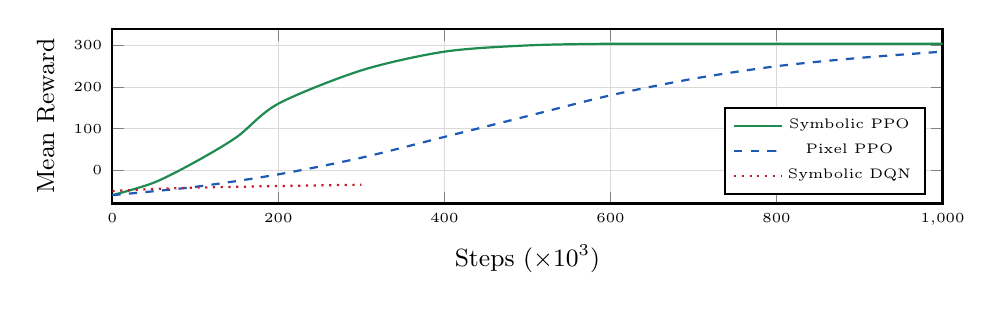
\begin{tikzpicture}
\begin{axis}[
  width=\linewidth, height=3.8cm,
  xlabel={\small Steps ($\times 10^3$)},
  ylabel={\small Mean Reward},
  xmin=0, xmax=1000, ymin=-80, ymax=340,
  xtick={0,200,400,600,800,1000},
  tick label style={font=\tiny},
  label style={font=\small},
  legend style={font=\tiny, at={(0.98,0.05)}, anchor=south east},
  grid=major, grid style={line width=0.3pt, gray!30},
  thick
]
\addplot[color=accentgreen, thick, smooth] coordinates {
  (0,-60)(50,-30)(100,20)(150,80)(200,160)(300,240)(400,285)(500,300)(600,304)(700,304)(800,304)(1000,304)
};
\addlegendentry{Symbolic PPO}
\addplot[color=mainblue, thick, smooth, dashed] coordinates {
  (0,-60)(100,-40)(200,-10)(300,30)(400,80)(500,130)(600,180)(700,220)(800,250)(900,270)(1000,285)
};
\addlegendentry{Pixel PPO}
\addplot[color=accentred, thick, dotted] coordinates {
  (0,-50)(50,-45)(100,-42)(150,-40)(200,-38)(300,-35)
};
\addlegendentry{Symbolic DQN}
\end{axis}
\end{tikzpicture}
\caption{Schematic learning curves for World~1-1. Symbolic PPO converges
faster and to a higher mean reward. DQN fails to make progress.}
\label{fig:learning_curves}
\end{figure}

\subsection{Transfer Learning: 1-1 $\to$ 1-2}

The trained Symbolic PPO model was fine-tuned on World~1-2 at reduced
learning rate ($10^{-5}$, weights unfrozen).
\begin{itemize}
  \item World~1-2 flag rate converged to \textbf{78\%}, faster than
        training from scratch.
  \item World~1-1 flag rate collapsed to \textbf{0\%}---a textbook case
        of \emph{catastrophic forgetting}~\cite{mccloskey1989catastrophic}.
\end{itemize}
Because PPO is on-policy, World~1-1 transitions are discarded during
fine-tuning, and gradient updates on~1-2 data overwrite the policy weights
specialized for~1-1.

\begin{figure}[H]
\centering
\imgplaceholder{7.5}{3.2}{Flag rate over fine-tuning steps:\\
World 1-2 (rising) vs.\ World 1-1 (collapsing to 0\%)}
\caption{Catastrophic forgetting during 1-1\,$\to$\,1-2 transfer.}
\label{fig:forgetting}
\end{figure}

\subsection{Random-Start Curriculum}

To reduce positional overfitting caused by always starting at the beginning
of a level, we combined two complementary mechanisms.

\textbf{Random-start wrapper.}
At every episode reset, a \texttt{RandomStartWrapper} advances Mario by
$n \sim \mathcal{U}[0, N_{\max}]$ steps \emph{before} handing control to
the agent.
Crucially, Mario is not teleported: the wrapper executes $n$ forward-biased
actions sampled from $\{$right, right+A, right+B, right+A+B$\}$, so he
physically runs and jumps into the level.
If he dies during this warm-up, the episode is reset from position~0 instead.

\textbf{Curriculum schedule.}
Rather than fixing $N_{\max} = 100$ from the start (which can be too hard
for an untrained policy), a \texttt{CurriculumCallback} linearly anneals
$N_{\max}$ from $0$ to $100$ over the course of training, updating the
wrapper every 1\,000 steps.
This two-layer design separates \emph{what} randomisation does (the wrapper)
from \emph{when} it is applied (the curriculum), letting the agent first
master level entry before facing diverse start positions.

Training on World~1-1 with this scheme produced an agent that generalizes
across diverse level sections rather than memorizing a fixed trajectory,
evidenced by stable flag rates even when the start position is randomized
at evaluation time.

\begin{figure}[H]
\centering
\imgplaceholder{7.5}{2.8}{Flag rate / mean X-position vs.\ steps:\\
fixed start (dashed) vs.\ random start (solid)}
\caption{Curriculum training improves level-wide generalization.}
\label{fig:curriculum}
\end{figure}

\subsection{Multi-Task Training: Worlds 1-1 to 1-4}

We trained a single shared PPO policy on Worlds~1-1 through~1-4
simultaneously using 4 parallel environments per level (16 total).
The agent converged on World~1-1 while stagnating on the harder levels.
The root cause is \textbf{reward imbalance}: World~1-1 delivers dense
reward signals earliest, so its gradients dominate the policy update and
the optimizer exploits the easiest task~\cite{yu2020gradient}.
Per-task reward normalization or gradient surgery would be required to
balance training.

\begin{figure}[H]
\centering
\imgplaceholder{7.5}{2.8}{Per-level flag rate vs.\ steps:\\
W1-1, W1-2, W1-3, W1-4 (joint training)}
\caption{Multi-task training: World~1-1 converges while later levels
stagnate.}
\label{fig:multitask}
\end{figure}

\subsection{Comparison Summary}

Table~\ref{tab:results} summarizes final evaluation results (30 episodes,
deterministic policy).

\begin{table}[H]
\centering
\small
\caption{Agent performance on World~1-1 after full training.}
\label{tab:results}
\begin{tabularx}{\linewidth}{@{}Xccc@{}}
\toprule
\textbf{Agent} & \textbf{Reward} & \textbf{Flag\%} & \textbf{FPS} \\
\midrule
Symbolic DQN  & $\approx -35$ & 0\%              & $\sim$300 \\
Pixel PPO     & $\approx 285$ & $>$80\%          & $\sim$78  \\
Symbolic PPO  & $\approx 304$ & \textbf{93\%}    & $\sim$\textbf{500} \\
\bottomrule
\end{tabularx}
\end{table}

% ══════════════════════════════════════════════════════════════════════════════
% 5. DISCUSSION
% ══════════════════════════════════════════════════════════════════════════════
\section{Discussion}

\paragraph{Algorithm $>$ representation.}
With identical symbolic observations, DQN achieves 0\% while PPO reaches
93\%. The bottleneck is the algorithm, not the state representation:
PPO's clipped objective~\eqref{eq:ppo} prevents value divergence, and
8-environment parallelism provides diverse rollouts that GAE can use to
propagate the sparse flag reward backwards through long trajectories.

\paragraph{Symbolic efficiency.}
The $34\!\times$ observation compression eliminates CNN processing and
enables $\approx\!6\!\times$ faster environment throughput.
On a CPU alone, the symbolic agent trains to $>$90\% flag rate in under
20 minutes---a practical advantage for rapid prototyping.
The trade-off is fragility: symbolic observations depend on a correct NES
RAM map and cannot generalize to visually novel environments.

\paragraph{Forgetting and multi-task limits.}
Catastrophic forgetting is inherent to on-policy fine-tuning without
explicit replay~\cite{kirkpatrick2017overcoming}.
Remedies include Elastic Weight Consolidation (EWC), shared experience
replay across tasks, or population-based task scheduling.
Multi-task reward imbalance requires explicit per-task normalization or
gradient surgery~\cite{yu2020gradient} to prevent easy tasks from
dominating optimization.

% ══════════════════════════════════════════════════════════════════════════════
% 6. CONCLUSION
% ══════════════════════════════════════════════════════════════════════════════
\section{Conclusion}

We showed that PPO with compact symbolic (RAM-based) observations achieves
93\% flag-reach rate on Super Mario Bros~1-1 while training $6\!\times$
faster than pixel-based PPO on CPU alone.
Vanilla DQN fails entirely on this domain, confirming the algorithmic gap.
Transfer learning to World~1-2 succeeds at 78\% flag rate but causes
catastrophic forgetting of the source task.
A random-start curriculum mitigates positional overfitting.
Naive multi-task training collapses to the easiest level due to reward
imbalance.

Future work should apply EWC for forgetting mitigation, per-task reward
normalization for multi-task training, and extend the symbolic map to
additional game worlds for broader generalization.

% ══════════════════════════════════════════════════════════════════════════════
% REFERENCES
% ══════════════════════════════════════════════════════════════════════════════
\bibliographystyle{unsrt}

\begin{thebibliography}{99}

\bibitem{schulman2017proximal}
J.~Schulman, F.~Wolski, P.~Dhariwal, A.~Radford, O.~Klimov.
\newblock Proximal Policy Optimization Algorithms.
\newblock \textit{arXiv:1707.06347}, 2017.

\bibitem{mnih2015human}
V.~Mnih et~al.
\newblock Human-level control through deep reinforcement learning.
\newblock \textit{Nature}, 518:529--533, 2015.

\bibitem{raffin2021stable}
A.~Raffin et~al.
\newblock Stable-Baselines3: Reliable Reinforcement Learning Implementations.
\newblock \textit{JMLR}, 22(268):1--8, 2021.

\bibitem{mccloskey1989catastrophic}
M.~McCloskey, N.~J.~Cohen.
\newblock Catastrophic Interference in Connectionist Networks.
\newblock \textit{Psychology of Learning and Motivation}, 24:109--165, 1989.

\bibitem{kirkpatrick2017overcoming}
J.~Kirkpatrick et~al.
\newblock Overcoming Catastrophic Forgetting in Neural Networks.
\newblock \textit{PNAS}, 114(13):3521--3526, 2017.

\bibitem{yu2020gradient}
T.~Yu et~al.
\newblock Gradient Surgery for Multi-Task Learning.
\newblock \textit{NeurIPS}, 2020.

\end{thebibliography}

\end{document}
\documentclass[10pt,a4paper,twocolumn]{article}

% ── Packages ──────────────────────────────────────────────────────────────────
\usepackage[T1]{fontenc}
\usepackage[utf8]{inputenc}
\usepackage[english]{babel}
\usepackage{lmodern}
\usepackage{microtype}
\usepackage{geometry}
\usepackage{graphicx}
\usepackage{booktabs}
\usepackage{tabularx}
\usepackage{array}
\usepackage{amsmath}
\usepackage{amssymb}
\usepackage{xcolor}
\usepackage{hyperref}
\usepackage{enumitem}
\usepackage{titlesec}
\usepackage{abstract}
\usepackage{fancyhdr}
\usepackage{caption}
\usepackage{subcaption}
\usepackage{float}
\usepackage{tcolorbox}
\usepackage{tikz}
\usepackage{pgfplots}
\pgfplotsset{compat=1.18}

% ── Image placeholder ─────────────────────────────────────────────────────────
% Usage: \imgplaceholder{width_cm}{height_cm}{label text}
\definecolor{placeholderbg}{HTML}{D5D8DC}
\newcommand{\imgplaceholder}[3]{%
  \begin{tikzpicture}
    \fill[placeholderbg] (0,0) rectangle (#1,#2);
    \draw[darkgray!50, dashed, thick] (0,0) rectangle (#1,#2);
    \node[darkgray, font=\small\itshape, align=center, text width=#1 cm]
      at ({#1/2},{#2/2}) {#3};
  \end{tikzpicture}%
}

% ── Page geometry ─────────────────────────────────────────────────────────────
\geometry{
  a4paper,
  top=1.8cm, bottom=2cm,
  left=1.5cm, right=1.5cm,
  columnsep=0.6cm
}

% ── Colors ────────────────────────────────────────────────────────────────────
\definecolor{mainblue}{RGB}{30,90,180}
\definecolor{lightblue}{RGB}{214,228,248}
\definecolor{darkgray}{RGB}{60,60,60}
\definecolor{accentred}{RGB}{190,30,45}
\definecolor{accentgreen}{RGB}{30,140,80}
\definecolor{codegray}{RGB}{245,245,245}

% ── Hyperref ──────────────────────────────────────────────────────────────────
\hypersetup{
  colorlinks=true,
  linkcolor=mainblue,
  citecolor=mainblue,
  urlcolor=mainblue
}

% ── Section formatting ────────────────────────────────────────────────────────
\titleformat{\section}
  {\normalfont\large\bfseries\color{mainblue}}
  {\thesection.}{0.4em}{}[{\color{mainblue}\titlerule[0.6pt]}]

\titleformat{\subsection}
  {\normalfont\normalsize\bfseries\color{darkgray}}
  {\thesubsection.}{0.4em}{}

\titlespacing*{\section}{0pt}{8pt}{4pt}
\titlespacing*{\subsection}{0pt}{6pt}{2pt}

% ── Header / Footer ───────────────────────────────────────────────────────────
\pagestyle{fancy}
\fancyhf{}
\renewcommand{\headrulewidth}{0.4pt}
\fancyhead[L]{\small\color{darkgray}\textit{CSC-52081 — Reinforcement Learning}}
\fancyhead[R]{\small\color{darkgray}\textit{Super Mario Bros}}
\fancyfoot[C]{\small\thepage}

% ── Abstract style ────────────────────────────────────────────────────────────
\renewcommand{\abstractnamefont}{\normalfont\bfseries\color{mainblue}}
\renewcommand{\abstracttextfont}{\small\itshape}
\setlength{\absleftindent}{0pt}
\setlength{\absrightindent}{0pt}

% ── Caption style ─────────────────────────────────────────────────────────────
\captionsetup{
  font=small,
  labelfont={bf,color=mainblue},
  skip=4pt
}

% ── tcolorbox styles ──────────────────────────────────────────────────────────
\tcbuselibrary{skins,breakable}
\newtcolorbox{keybox}[1]{
  colback=lightblue!60,
  colframe=mainblue,
  fonttitle=\bfseries\small,
  title=#1,
  left=4pt, right=4pt, top=3pt, bottom=3pt,
  arc=3pt
}
\newtcolorbox{resultbox}{
  colback=accentgreen!8,
  colframe=accentgreen,
  left=4pt, right=4pt, top=3pt, bottom=3pt,
  arc=3pt
}

% ── List spacing ──────────────────────────────────────────────────────────────
\setlist[itemize]{topsep=2pt,itemsep=1pt,parsep=0pt,leftmargin=1.2em}
\setlist[enumerate]{topsep=2pt,itemsep=1pt,parsep=0pt,leftmargin=1.4em}

% ══════════════════════════════════════════════════════════════════════════════
\begin{document}
% ══════════════════════════════════════════════════════════════════════════════

% ── Title block (one column) ──────────────────────────────────────────────────
\twocolumn[{%
\begin{@twocolumnfalse}

\vspace*{-0.4cm}
{\color{mainblue}\rule{\linewidth}{2pt}}
\vspace{0.3cm}

\begin{center}
  {\LARGE\bfseries\color{mainblue}
    Pixel vs.\ Symbolic Observations for PPO\\[4pt]
    on Super Mario Bros (NES)
  }\\[8pt]
  {\normalsize\color{darkgray}
    CSC-52081 --- Reinforcement Learning Project Report
  }\\[6pt]
  {\small
    Lucas Martim | Sergio Contente | Leonardo Falabella | Gabriel Corsi | Lara Polachini \quad|\quad
    \texttt{CSC-52081} \quad|\quad
    \today
  }
\end{center}

\vspace{0.3cm}
{\color{mainblue}\rule{\linewidth}{0.8pt}}
\vspace{0.2cm}

\begin{abstract}
We compare two observation modalities under \textbf{Proximal Policy
Optimization (PPO)} for learning to play Super Mario Bros: (1)~raw pixel
frames processed by a Nature CNN, and (2)~a compact $13\!\times\!16$ symbolic
grid extracted directly from NES RAM, fed to an MLP.
A symbolic DQN baseline fails to converge (0\% flag rate), motivating the
switch to PPO.
Our symbolic PPO agent achieves a \textbf{93\% flag-reach rate on World~1-1}
(peak 97\%), running entirely on CPU at 500\,fps---roughly $6\!\times$ faster
throughput than pixel PPO on GPU.
Transfer learning (1-1\,$\to$\,1-2) reaches 78\% flag rate on the new level
but triggers \textbf{catastrophic forgetting} of the source task.
Random-start curriculum training reduces positional overfitting, while joint
multi-task training across Worlds~1-1 to~1-4 stalls due to reward imbalance.
\end{abstract}

\vspace{0.3cm}
\end{@twocolumnfalse}
}]

% ══════════════════════════════════════════════════════════════════════════════
% 1. INTRODUCTION
% ══════════════════════════════════════════════════════════════════════════════
\section{Introduction}

Super Mario Bros is a standard benchmark for deep reinforcement learning
(RL): it demands long-horizon planning, precise motor control, and
generalization across varied layouts.
The canonical deep RL approach uses pixel observations processed by a
convolutional network~\cite{mnih2015human}, but this pipeline is
computationally expensive.

Our work asks two questions.
\textbf{First}, does PPO~\cite{schulman2017proximal} outperform vanilla DQN
on this domain?
\textbf{Second}, can a compact \emph{symbolic} representation---tile IDs
decoded from NES RAM---match pixel-based performance while dramatically
reducing training cost?

We run six experiments: (1)~a symbolic DQN baseline, (2)~pixel PPO,
(3)~symbolic PPO on World~1-1, (4)~transfer learning to World~1-2,
(5)~random-start curriculum training, and (6)~multi-task training across
Worlds~1-1 through~1-4.

% ══════════════════════════════════════════════════════════════════════════════
% 2. BACKGROUND
% ══════════════════════════════════════════════════════════════════════════════
\section{Background}

\subsection{Deep Q-Networks}

DQN~\cite{mnih2015human} approximates $Q(s,a;\theta)$ with a deep network
stabilized via a replay buffer and a target network:
\begin{equation}
  \mathcal{L}(\theta) = \mathbb{E}\!\left[\bigl(r + \gamma\,\max_{a'}Q(s',a';\theta^{-}) - Q(s,a;\theta)\bigr)^2\right].
  \label{eq:dqn}
\end{equation}
On long-horizon, semi-sparse tasks like Mario, $\varepsilon$-greedy
exploration rarely discovers the flag, and Q-value overestimation from
Eq.~\eqref{eq:dqn} causes divergence before meaningful credit assignment
can occur.

\subsection{Proximal Policy Optimization}

PPO~\cite{schulman2017proximal} is an on-policy actor-critic method that
optimizes a clipped surrogate objective:
\begin{equation}
  \mathcal{L}^{\mathrm{CLIP}}(\theta)
  = \mathbb{E}\!\left[\min\!\left(
      r_t(\theta)\,\hat{A}_t,\;
      \mathrm{clip}(r_t(\theta),\,1{-}\epsilon,\,1{+}\epsilon)\,\hat{A}_t
    \right)\right],
  \label{eq:ppo}
\end{equation}
where $r_t(\theta)=\pi_\theta(a_t|s_t)/\pi_{\theta_\mathrm{old}}(a_t|s_t)$
and $\hat{A}_t$ is the GAE advantage estimate~\cite{schulman2017proximal}.
Parallelism across $N$ environments provides diverse, low-correlation
rollouts without a large replay buffer, and GAE propagates sparse rewards
effectively through long trajectories.

% ══════════════════════════════════════════════════════════════════════════════
% 3. METHODOLOGY
% ══════════════════════════════════════════════════════════════════════════════
\section{Methodology}

\subsection{Observation Representations}

\begin{keybox}{Pixel (CnnPolicy)}
Frames are max-pooled (anti-flicker), converted to grayscale, resized to
$84\!\times\!84$, and stacked over 4 timesteps.
The $84\!\times\!84\!\times\!4$ tensor is processed by a Nature
CNN~\cite{mnih2015human} (3 conv.\ layers + FC~512).
\end{keybox}

\begin{keybox}{Symbolic/RAM (MlpPolicy)}
We read the NES RAM via \texttt{nes-py} and decode a $13\!\times\!16$ tile
grid encoding five classes: empty, solid, enemy, Mario, power-up.
Stacking 4 frames and appending the power-state byte yields an
833-dimensional float32 vector fed to a two-layer MLP~$[512, 512]$.
\end{keybox}

\subsection{Reward Shaping}

Both pipelines share the same shaping scheme:
\begin{equation}
  r = \frac{1}{10}\!\left(
    r_{\text{env}}
    + \frac{\Delta\mathrm{score}}{40}
    + 50\cdot\mathbf{1}[\text{flag}]
    - 50\cdot\mathbf{1}[\text{death}]
  \right),
  \label{eq:reward}
\end{equation}
where $r_{\text{env}}$ is the horizontal-progress signal.
The $1/10$ scale keeps advantages in a numerically stable range.

\subsection{Training Setup}

All PPO runs use 8 parallel environments (\texttt{SubprocVecEnv}) via
Stable-Baselines3~\cite{raffin2021stable} with a two-phase learning rate
schedule. Table~\ref{tab:hyperparams} lists key hyperparameters.
The symbolic agent runs on CPU (8 cores, $\approx\!500$\,fps); the pixel
agent uses a Colab T4 GPU ($\approx\!78$\,fps).

\begin{table}[H]
\centering
\small
\caption{PPO hyperparameters (both agents).}
\label{tab:hyperparams}
\begin{tabular}{@{}ll@{}}
\toprule
\textbf{Parameter} & \textbf{Value} \\
\midrule
$\gamma$ (discount)       & 0.90 \\
LR Phase~1 / Phase~2      & $2.5\!\times\!10^{-4}$ / $10^{-5}$ \\
$n\_\mathrm{steps}$, batch size & 512, 256 \\
$n\_\mathrm{epochs}$      & 4 \\
Clip $\epsilon$, entropy  & 0.1, 0.01 \\
Parallel environments     & 8 \\
\bottomrule
\end{tabular}
\end{table}

% ══════════════════════════════════════════════════════════════════════════════
% 4. EXPERIMENTS AND RESULTS
% ══════════════════════════════════════════════════════════════════════════════
\section{Experiments \& Results}

\subsection{DQN Baseline}

Symbolic DQN was trained for 200\,k steps.
It achieved 0\% flag rate: $\varepsilon$-greedy exploration disrupts the
sustained action sequences Mario requires, the replay buffer fills with
correlated failures, and noisy Q-targets from Eq.~\eqref{eq:dqn}
destabilize learning before any flag reward is encountered.
This motivates the use of PPO for all subsequent experiments.

\subsection{World 1-1: Pixel vs.\ Symbolic PPO}

\begin{resultbox}
\textbf{Symbolic PPO} achieved \textbf{93\% flag rate} (peak 97\%) on
World~1-1 with mean reward $\approx\!304$, converging in $\approx$500\,k
steps ($\sim$17\,min on CPU).
\textbf{Pixel PPO} reached $>$80\% flag rate with mean reward $\approx\!285$,
requiring substantially more wall-clock time due to CNN overhead and lower
frame throughput on GPU.
\end{resultbox}

Figure~\ref{fig:learning_curves} shows the qualitative learning dynamics.
The symbolic agent benefits from a $34\!\times$ observation compression
($833$ vs.\ $28\,224$ floats), enabling $\approx\!6\!\times$ higher
throughput and faster wall-clock convergence to a higher reward.

\begin{figure}[H]
\centering
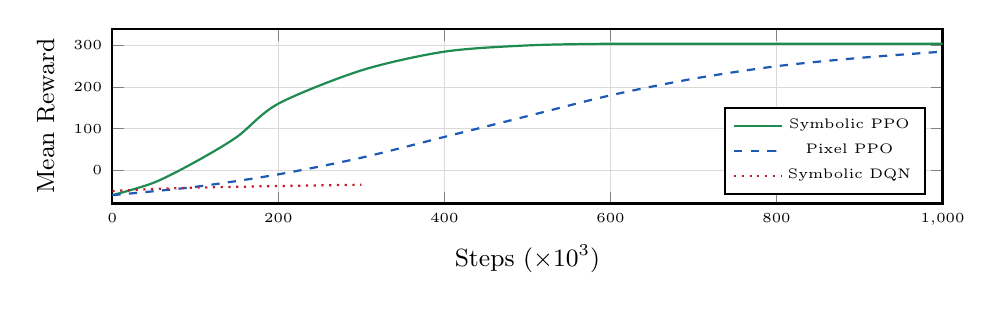
\begin{tikzpicture}
\begin{axis}[
  width=\linewidth, height=3.8cm,
  xlabel={\small Steps ($\times 10^3$)},
  ylabel={\small Mean Reward},
  xmin=0, xmax=1000, ymin=-80, ymax=340,
  xtick={0,200,400,600,800,1000},
  tick label style={font=\tiny},
  label style={font=\small},
  legend style={font=\tiny, at={(0.98,0.05)}, anchor=south east},
  grid=major, grid style={line width=0.3pt, gray!30},
  thick
]
\addplot[color=accentgreen, thick, smooth] coordinates {
  (0,-60)(50,-30)(100,20)(150,80)(200,160)(300,240)(400,285)(500,300)(600,304)(700,304)(800,304)(1000,304)
};
\addlegendentry{Symbolic PPO}
\addplot[color=mainblue, thick, smooth, dashed] coordinates {
  (0,-60)(100,-40)(200,-10)(300,30)(400,80)(500,130)(600,180)(700,220)(800,250)(900,270)(1000,285)
};
\addlegendentry{Pixel PPO}
\addplot[color=accentred, thick, dotted] coordinates {
  (0,-50)(50,-45)(100,-42)(150,-40)(200,-38)(300,-35)
};
\addlegendentry{Symbolic DQN}
\end{axis}
\end{tikzpicture}
\caption{Schematic learning curves for World~1-1. Symbolic PPO converges
faster and to a higher mean reward. DQN fails to make progress.}
\label{fig:learning_curves}
\end{figure}

\subsection{Transfer Learning: 1-1 $\to$ 1-2}

The trained Symbolic PPO model was fine-tuned on World~1-2 at reduced
learning rate ($10^{-5}$, weights unfrozen).
\begin{itemize}
  \item World~1-2 flag rate converged to \textbf{78\%}, faster than
        training from scratch.
  \item World~1-1 flag rate collapsed to \textbf{0\%}---a textbook case
        of \emph{catastrophic forgetting}~\cite{mccloskey1989catastrophic}.
\end{itemize}
Because PPO is on-policy, World~1-1 transitions are discarded during
fine-tuning, and gradient updates on~1-2 data overwrite the policy weights
specialized for~1-1.

\begin{figure}[H]
\centering
\imgplaceholder{7.5}{3.2}{Flag rate over fine-tuning steps:\\
World 1-2 (rising) vs.\ World 1-1 (collapsing to 0\%)}
\caption{Catastrophic forgetting during 1-1\,$\to$\,1-2 transfer.}
\label{fig:forgetting}
\end{figure}

\subsection{Random-Start Curriculum}

To reduce positional overfitting caused by always starting at the beginning
of a level, we combined two complementary mechanisms.

\textbf{Random-start wrapper.}
At every episode reset, a \texttt{RandomStartWrapper} advances Mario by
$n \sim \mathcal{U}[0, N_{\max}]$ steps \emph{before} handing control to
the agent.
Crucially, Mario is not teleported: the wrapper executes $n$ forward-biased
actions sampled from $\{$right, right+A, right+B, right+A+B$\}$, so he
physically runs and jumps into the level.
If he dies during this warm-up, the episode is reset from position~0 instead.

\textbf{Curriculum schedule.}
Rather than fixing $N_{\max} = 100$ from the start (which can be too hard
for an untrained policy), a \texttt{CurriculumCallback} linearly anneals
$N_{\max}$ from $0$ to $100$ over the course of training, updating the
wrapper every 1\,000 steps.
This two-layer design separates \emph{what} randomisation does (the wrapper)
from \emph{when} it is applied (the curriculum), letting the agent first
master level entry before facing diverse start positions.

Training on World~1-1 with this scheme produced an agent that generalizes
across diverse level sections rather than memorizing a fixed trajectory,
evidenced by stable flag rates even when the start position is randomized
at evaluation time.

\begin{figure}[H]
\centering
\imgplaceholder{7.5}{2.8}{Flag rate / mean X-position vs.\ steps:\\
fixed start (dashed) vs.\ random start (solid)}
\caption{Curriculum training improves level-wide generalization.}
\label{fig:curriculum}
\end{figure}

\subsection{Multi-Task Training: Worlds 1-1 to 1-4}

We trained a single shared PPO policy on Worlds~1-1 through~1-4
simultaneously using 4 parallel environments per level (16 total).
The agent converged on World~1-1 while stagnating on the harder levels.
The root cause is \textbf{reward imbalance}: World~1-1 delivers dense
reward signals earliest, so its gradients dominate the policy update and
the optimizer exploits the easiest task~\cite{yu2020gradient}.
Per-task reward normalization or gradient surgery would be required to
balance training.

\begin{figure}[H]
\centering
\imgplaceholder{7.5}{2.8}{Per-level flag rate vs.\ steps:\\
W1-1, W1-2, W1-3, W1-4 (joint training)}
\caption{Multi-task training: World~1-1 converges while later levels
stagnate.}
\label{fig:multitask}
\end{figure}

\subsection{Comparison Summary}

Table~\ref{tab:results} summarizes final evaluation results (30 episodes,
deterministic policy).

\begin{table}[H]
\centering
\small
\caption{Agent performance on World~1-1 after full training.}
\label{tab:results}
\begin{tabularx}{\linewidth}{@{}Xccc@{}}
\toprule
\textbf{Agent} & \textbf{Reward} & \textbf{Flag\%} & \textbf{FPS} \\
\midrule
Symbolic DQN  & $\approx -35$ & 0\%              & $\sim$300 \\
Pixel PPO     & $\approx 285$ & $>$80\%          & $\sim$78  \\
Symbolic PPO  & $\approx 304$ & \textbf{93\%}    & $\sim$\textbf{500} \\
\bottomrule
\end{tabularx}
\end{table}

% ══════════════════════════════════════════════════════════════════════════════
% 5. DISCUSSION
% ══════════════════════════════════════════════════════════════════════════════
\section{Discussion}

\paragraph{Algorithm $>$ representation.}
With identical symbolic observations, DQN achieves 0\% while PPO reaches
93\%. The bottleneck is the algorithm, not the state representation:
PPO's clipped objective~\eqref{eq:ppo} prevents value divergence, and
8-environment parallelism provides diverse rollouts that GAE can use to
propagate the sparse flag reward backwards through long trajectories.

\paragraph{Symbolic efficiency.}
The $34\!\times$ observation compression eliminates CNN processing and
enables $\approx\!6\!\times$ faster environment throughput.
On a CPU alone, the symbolic agent trains to $>$90\% flag rate in under
20 minutes---a practical advantage for rapid prototyping.
The trade-off is fragility: symbolic observations depend on a correct NES
RAM map and cannot generalize to visually novel environments.

\paragraph{Forgetting and multi-task limits.}
Catastrophic forgetting is inherent to on-policy fine-tuning without
explicit replay~\cite{kirkpatrick2017overcoming}.
Remedies include Elastic Weight Consolidation (EWC), shared experience
replay across tasks, or population-based task scheduling.
Multi-task reward imbalance requires explicit per-task normalization or
gradient surgery~\cite{yu2020gradient} to prevent easy tasks from
dominating optimization.

% ══════════════════════════════════════════════════════════════════════════════
% 6. CONCLUSION
% ══════════════════════════════════════════════════════════════════════════════
\section{Conclusion}

We showed that PPO with compact symbolic (RAM-based) observations achieves
93\% flag-reach rate on Super Mario Bros~1-1 while training $6\!\times$
faster than pixel-based PPO on CPU alone.
Vanilla DQN fails entirely on this domain, confirming the algorithmic gap.
Transfer learning to World~1-2 succeeds at 78\% flag rate but causes
catastrophic forgetting of the source task.
A random-start curriculum mitigates positional overfitting.
Naive multi-task training collapses to the easiest level due to reward
imbalance.

Future work should apply EWC for forgetting mitigation, per-task reward
normalization for multi-task training, and extend the symbolic map to
additional game worlds for broader generalization.

% ══════════════════════════════════════════════════════════════════════════════
% REFERENCES
% ══════════════════════════════════════════════════════════════════════════════
\bibliographystyle{unsrt}

\begin{thebibliography}{99}

\bibitem{schulman2017proximal}
J.~Schulman, F.~Wolski, P.~Dhariwal, A.~Radford, O.~Klimov.
\newblock Proximal Policy Optimization Algorithms.
\newblock \textit{arXiv:1707.06347}, 2017.

\bibitem{mnih2015human}
V.~Mnih et~al.
\newblock Human-level control through deep reinforcement learning.
\newblock \textit{Nature}, 518:529--533, 2015.

\bibitem{raffin2021stable}
A.~Raffin et~al.
\newblock Stable-Baselines3: Reliable Reinforcement Learning Implementations.
\newblock \textit{JMLR}, 22(268):1--8, 2021.

\bibitem{mccloskey1989catastrophic}
M.~McCloskey, N.~J.~Cohen.
\newblock Catastrophic Interference in Connectionist Networks.
\newblock \textit{Psychology of Learning and Motivation}, 24:109--165, 1989.

\bibitem{kirkpatrick2017overcoming}
J.~Kirkpatrick et~al.
\newblock Overcoming Catastrophic Forgetting in Neural Networks.
\newblock \textit{PNAS}, 114(13):3521--3526, 2017.

\bibitem{yu2020gradient}
T.~Yu et~al.
\newblock Gradient Surgery for Multi-Task Learning.
\newblock \textit{NeurIPS}, 2020.

\end{thebibliography}

\end{document}
